%!/usr/bin/pdflatex

% The French Pratham ground station software system
%
% Author : Hai Nguyen Van,
% Institut de Physique du Globe de Paris, Université Paris Diderot
%
% The copyright to this code is held by Institut de Physique du Globe de Paris. All rights reserved. This file is distributed under the license CeCILL Free Software License Agreement.


% Use the following line for draft mode (double spaced, single column)
%\documentclass[preprint,pre,floats,aps,amsmath,amssymb]{revtex4}

% Use the following line for journal mode (single spaced, double column)
\documentclass[a4paper]{report}
%\documentclass[twocolumn,pre,floats,aps,amsmath,amssymb]{revtex4}
\usepackage{graphicx}
\usepackage{bm}
\usepackage{color}
\usepackage{multirow}
\usepackage{version}
\usepackage{hyperref}
\usepackage{algorithm}
\usepackage{algorithmic}
\usepackage{amssymb}
\usepackage{amsmath}
\usepackage{marvosym}
\usepackage{rotating}
%\usepackage[final]{pdfpages}
\usepackage{tikz}
\usepackage[top=2cm, bottom=2cm, left=2cm, right=2cm]{geometry}
\usetikzlibrary{automata,positioning}

%%%%%%%%%%%%%%%%%%%%%%%%%%%%%%%%%%%%%%%%%%%%%%%%%%%%%%%%%%%%%%%%%%%%%%%%%%%%%
\newtheorem{theorem}{Theorem.}[section]
\newtheorem{lemma}[theorem]{Lemma.}
\newtheorem{proposition}[theorem]{Lemma.}
\newtheorem{corollary}[theorem]{Corollary.}
%\newtheorem{algorithm}[theorem]{Algorithme.}

\newenvironment{implementation}[1][Impl\'ementation.]{\begin{trivlist}
\item[\hskip \labelsep {\bfseries #1}]}{\end{trivlist}}

\newenvironment{proof}[1][Proof.]{\begin{trivlist}
\item[\hskip \labelsep {\bfseries #1}]}{\end{trivlist}}

\newenvironment{notation}[1][Notation.]{\begin{trivlist}
\item[\hskip \labelsep {\bfseries #1}]}{\end{trivlist}}


\newenvironment{definition}[1][Definition.]{\begin{trivlist}
\item[\hskip \labelsep {\bfseries #1}]}{\end{trivlist}}
\newenvironment{example}[1][Example.]{\begin{trivlist}
\item[\hskip \labelsep {\bfseries #1}]}{\end{trivlist}}
\newenvironment{remark}[1][Remark.]{\begin{trivlist}
\item[\hskip \labelsep {\bfseries #1}]}{\end{trivlist}}
%%%%%%%%%%%%%%%%%%%%%%%%%%%%%%%%%%%%%%%%%%%%%%%%%%%%%%%%%%%%%%%%%%%%%%%%%%%%%

\definecolor{rltgreen}{rgb}{0,0.5,0}
\definecolor{rltred}{rgb}{0.75,0,0}
\definecolor{grey}{rgb}{0.75,0.75,0.75}
\definecolor{oneblue}{rgb}{0,0,0.75}

\begin{document}

\title{The French Pratham ground station software system}

\author{\'Equipe Pratham, Universit\'e Paris Diderot, Institut de Physique du Globe de Paris}
%\affiliation{Universit\'e Paris Diderot $-$ Institut de Physique du Globe de Paris, 4 avenue de Neptune, 94100 Saint-Maur-des-Foss\'es, France}
\date{\today}

\maketitle

\tableofcontents




\chapter{Foreword}
\label{sec:foreword}

The following reference manual introduces technical issues related to the control-data-acquistion software system of the ground station at IPGP for Pratham satellite~\cite{IITB_general}. It aims to give scientific answers to the choice of implemented structures, including: antenna rotor control, time-based acquisition scheduler, \textsc{fsk} (\textsc{frequency-shift keying}) and \textsc{ook} (\textsc{on-off keying}) demodulation, \textsc{ax.25} frame decoding, \textsc{morse} code decoding and data recording.

\textbf{Warning.} Section marks { \color{rltred}{\Radioactivity} } give scientific arguments but not necessarily relevant information for the understanding of this document. Some algorithm implementation details have been omitted for more abstraction towards specific programming languages.

\section{Licensing}

The set of softwares provided as follows is copyright (c) 2010-2013 Institut de Physique du Globe de Paris (IPGP). IPGP holds all ownership rights to the software system.
The software system is open source and can be freely redistributed. See the file \verb!LICENSE! in the distribution for licensing information.
The present documentation is copyright (c) 2010-2013 Institut de Physique du Globe de Paris (IPGP). This reference manual may be reproduced and distributed in whole or in part, subject to the following conditions:
\begin{itemize}
\item The copyright notice above and this permission notice must be preserved complete on all complete or partial copies.
\item Any translation or derivative work of this reference manual must be approved by the authors in writing before distribution.
\item If you distribute this reference manual in part, instructions for obtaining the complete version of this manual must be included, and a means for obtaining a complete version provided.
\item Small portions may be reproduced as illustrations for reviews or quotes in other works without this permission notice if proper citation is given.
\end{itemize}

\section{Availability}

The complete set of softwares can be accessed via the Web site \verb!https://github.com/EmptyStackExn!.

\chapter{Introduction}
\label{sec:intro}
\section{Overview}

The \texttt{NI-6353}~\cite{NI_6353_datasheet}~\cite{NI_calibration_procedure} Acquisition Box (considered as an ADC) acquires twelve voltage measurements in volt (V).

\begin{table}[ht]
  \caption{Set of voltage measurements to acquire}
  \begin{center}
    \begin{footnotesize}
      \begin{tabular}{|c|c|c|rcc|}
        \hline
        \multirow{7}{*}{145,980 MHz antenna} & \multirow{3}{*}{Plane 1} & \multirow{3}{*}{$\dots$} & VR5000          & \color{rltgreen}{$\rightarrow$} & \multirow{14}{*}{NI-6353}\\ \cline{4-5}
        &                         &                          & AD8302$_{mag}$   & \color{oneblue}{$\rightarrow$} & \\ \cline{4-5}
        &                         &                          & AD8302$_{phase}$ & \color{oneblue}{$\rightarrow$} & \\ \cline{2-5}
        & \multirow{3}{*}{Plane 2} & \multirow{3}{*}{$\dots$} & VR5000          & \color{rltgreen}{$\rightarrow$} & \\ \cline{4-5}
        &                         &                          & AD8302$_{mag}$   & \color{oneblue}{$\rightarrow$} & \\ \cline{4-5}
        &                         &                          & AD8302$_{phase}$ & \color{oneblue}{$\rightarrow$} & \\ \cline{1-5}
        
        \multirow{7}{*}{437,455 MHz antenna} & \multirow{3}{*}{Plane 1} & \multirow{3}{*}{$\dots$} & VR5000          & \color{rltred}{$\rightarrow$}  & \\ \cline{4-5}
        &                         &                          & AD8302$_{mag}$   & \color{oneblue}{$\rightarrow$} & \\ \cline{4-5}
        &                         &                          & AD8302$_{phase}$ & \color{oneblue}{$\rightarrow$} & \\ \cline{2-5}
        & \multirow{3}{*}{Plane 2} & \multirow{3}{*}{$\dots$} & VR5000          & \color{rltred}{$\rightarrow$} & \\ \cline{4-5}
        &                         &                          & AD8302$_{mag}$   & \color{oneblue}{$\rightarrow$} & \\ \cline{4-5}
        &                         &                          & AD8302$_{phase}$ & \color{oneblue}{$\rightarrow$} & \\ \cline{4-5}
        
        \hline
      \end{tabular}
    \end{footnotesize}
  \end{center}
  \label{tab:diagramme_gen}
\end{table}

\begin{remark}
  We introduce on \textsc{table}~\ref{tab:diagramme_gen} a flowchart of acquisition channels at the input of ADC. { \color{oneblue}{Blue} } arrows ($\rightarrow$) match with channels from which the ADC acquire voltage measurements (in Volts). In the same way, { \color{rltgreen}{green} } (resp. { \color{rltred}{red} }) arrows match with as well voltage measurements acquisition as \textsc{ook} demodulation and \textsc{Morse} decoding (resp. \textsc{fsk} demodulation and \textsc{ax.25} frame decoding).
\end{remark}

\section{Digital signal at 437,455 MHz : Health monitoring data}

The following process is applied to the two channels specified by { \color{rltred}{red} } arrows of the previous flowchart. At the end of the process we then have two output files for the same information $-$ as a matter of fact $-$ more accuracy.

\begin{figure}[h]
  \begin{center}
  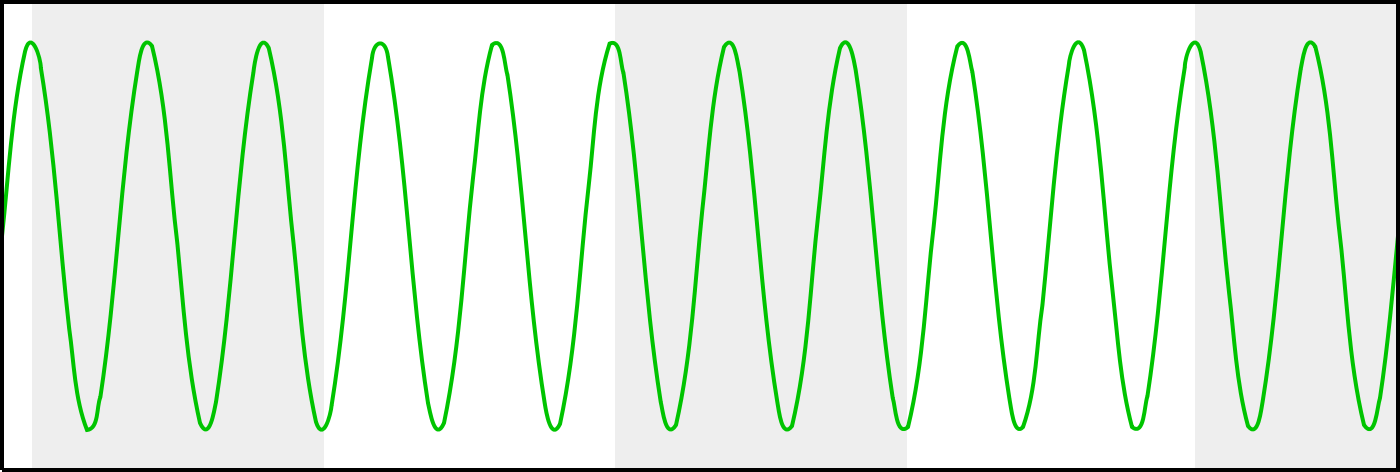
\includegraphics[width=8cm]{pictures/porteuse.png}
  \end{center}
  \caption{Carrier signal (central frequency $F_c$)}
  \label{fig:signal_porteur}
\end{figure}

\begin{figure}[h]
  \begin{center}
  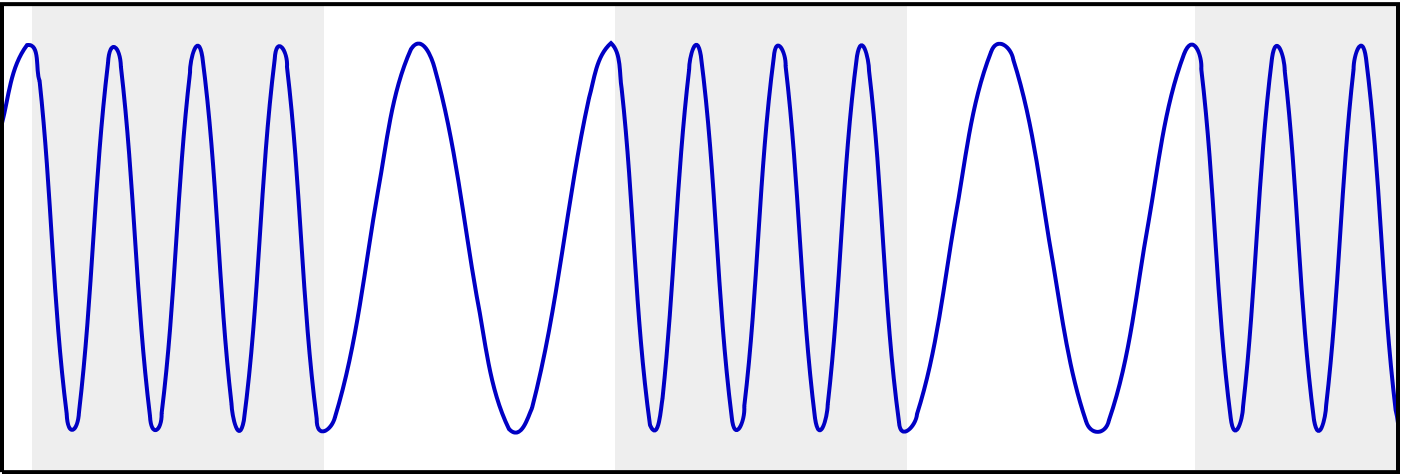
\includegraphics[width=8cm]{pictures/signal_mod.png}
  \end{center}
  \caption{Modulated signal in \textsc{fsk} at $F_c \pm \frac{\Delta f}{2}$ frequencies received by the \texttt{VR5000}}
  \label{fig:signal_module}
\end{figure}

\begin{figure}[h]
  \begin{center}
  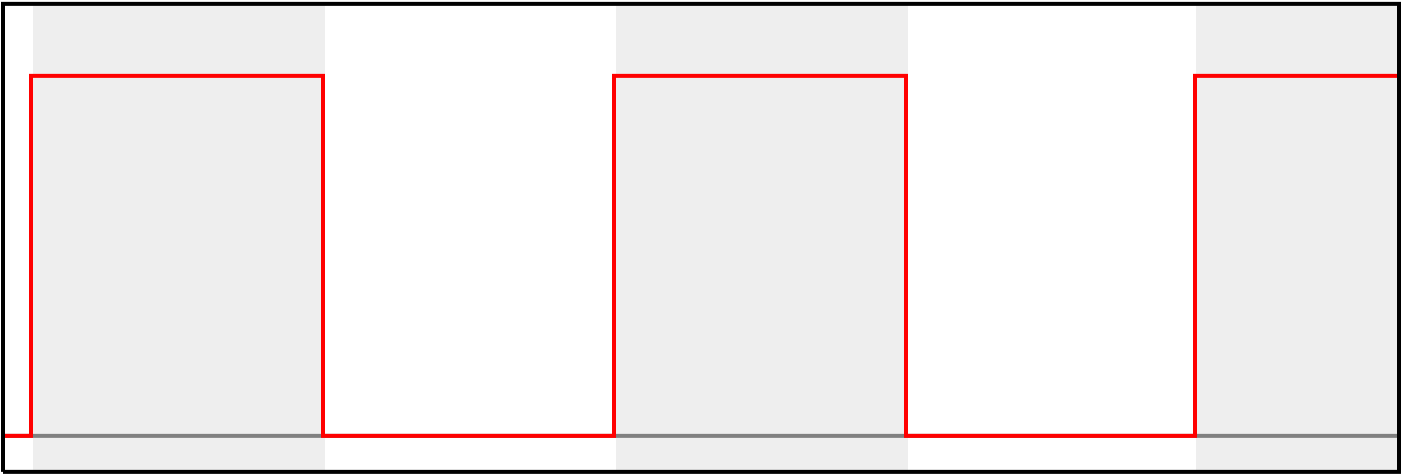
\includegraphics[width=8cm]{pictures/signal_demod.png}
  \end{center}
  \caption{Modulating signal at $F_b = 1,2 \ \operatorname{kbit}.\operatorname{s}^{-1}$ bit rate (retrieved by \textsc{fsk} demodulation)}
  \label{fig:signal_modulant}
\end{figure}

The satellite sends a signal with a declared carrier signal at $F_c = 437,455$ MHz (\textsc{figure}~\ref{fig:signal_porteur}) and a passband bandwidth of $\Delta f = 9,90$ kHz (ref ?). At the end of the acquisition chain the \textsc{vr5000} transceiver acquires a signal whose central frequency is $F_c$ and whose passband bandwidth is $\Delta f$ (\textsc{figure}~\ref{fig:signal_module}).

The transceiver returns an audio signal. It finally decribes $-$ through a Schmitt trigger (ref ?) $-$ the modulating signal (\textsc{figure}~\ref{fig:signal_modulant}). The digital baseband transmission method is of the kind non-return-to-zero (\textsc{nrz})~\cite{nrz_gorry} (ref ?). The data bits are then saved in a file (\textsc{figure}~\ref{fig:bits_donnees}) in such a way that (more info on peak sync ? method not sure...) on a time length $T_b$, the highest mean amplitude of a frequency would match its logical \texttt{0} or \texttt{1}.

%On termine la d\'emodulation \texttt{FSK} en calculant, par \textit{transform\'ee de Fourier}, les amplitudes associ\'ees aux composantes fr\'equentielles $0$ et $1,2$ kHz sur une largeur de fen\^etre de calcul $\Delta t = \frac{1}{F_b}$.

\begin{figure}[h]
  \begin{center}
  \begin{tabular}{|c|}
    \hline
    $\dots$
    \textcolor{rltred}{$\underbrace{\texttt{01111110}}_{\textup{packet start}}$}
    $\dots$
    \textcolor{rltgreen}{$\underbrace{\texttt{10101010}}_{\textup{information}}$}
    $\dots$
    \textcolor{rltred}{$\underbrace{\texttt{01111110}}_{\textup{packet end}}$}
    $\dots$\\
    \hline
  \end{tabular}
  \end{center}
\caption{Data bits associated to the modulating signal}
\label{fig:bits_donnees}
\end{figure}

We decode data bits from the \textsc{ax.25} data link layer protocol (\textsc{figure}~\ref{fig:bits_sans_ax25}).

\begin{figure}[h]
  \begin{center}
  \begin{tabular}{|c|}
    \hline
    $\dots$ \textcolor{rltgreen}{\texttt{10101010}} $\dots$\\
    \hline
  \end{tabular}
  \end{center}
  \caption{Data bits decoded from \texttt{AX.25} packets}
  \label{fig:bits_sans_ax25}
\end{figure}

At the end of the process we evaluate data bits as defined by \textsc{iitb}'s specification\cite{IITB}.

\newpage

\section{Digital signal at 145,980 MHz : Beacon}

In the same way the transceiver demodulates a signal of central frequency $F_c = 145,980$ MHz (\textsc{figure}~\ref{fig:signal_ook}). Considering a bit rate of $F_b = 10 \ \operatorname{bit}.\operatorname{s}^{-1}$, the presence of the amplitude associated to the frequency component $F_c$ matches with a pulse and the abscence with no pulse as specified by \textsc{on-off keying} (\textsc{figure}~\ref{fig:impulsions_morse}).

\begin{figure}[h]
  \begin{center}
  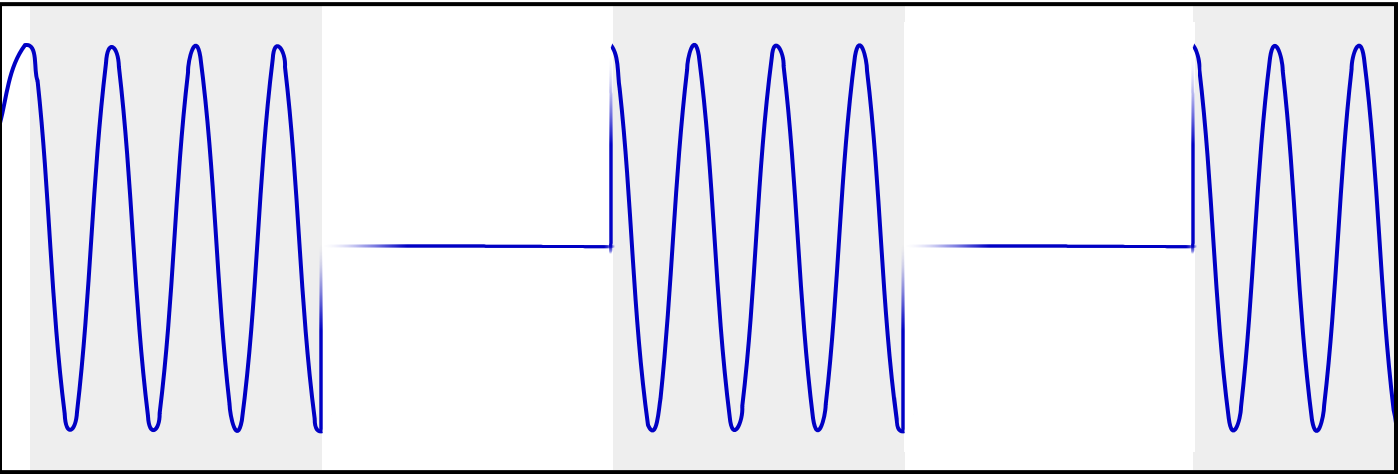
\includegraphics[width=8cm]{pictures/sans_porteuse.png}
  \end{center}
  \caption{Modulated signal in \textsc{ook} of fr\'equency $F_c$ received by the transceiver}
  \label{fig:signal_ook}
\end{figure}

We demodulate the digital baseband transmission method considering that a logical \texttt{1} matches with a pulse of a time length that equals to a \textsc{dit} with \textsc{dits}, \textsc{dah} and $\varepsilon$ (no impulse) (\textsc{figure}~\ref{fig:impulsions_morse}).

\begin{figure}[h]
  \begin{center}
  \begin{tabular}{|c|}
    \hline
    $\dots$ \textcolor{rltred}{\texttt{...- ..- ..--- -- -.. --.-}} $\dots$\\
    \hline
  \end{tabular}
  \end{center}
  \caption{Digitized signal associated to pulses}
  \label{fig:impulsions_morse}
\end{figure}

We finally decode \textsc{morse} to retrieve the information on two channels ({ \color{rltgreen}{green} } arrows on the previous flowchart). We have two files with the same information.

\begin{figure}[h]
  \begin{center}
  \begin{tabular}{|c|}
    \hline
    $\dots$ \textcolor{rltgreen}{\texttt{VU2MDQ}} $\dots$\\
    \hline
  \end{tabular}
  \end{center}
  \caption{\textsc{Morse} decoded information}
  \label{fig:info_decode_morse}
\end{figure}


\section{Gain and phase detection : TEC information}

Eight channels ({ \color{oneblue}{blue} } arrows on the previous flowchart) will allow us to acquire the \textsc{ad8302} Gain and Phase Detectors. We directly save voltage measurements in a file. \textsc{tec} retrieving will be done as post-processing with an external Matlab program.

\chapter{Acquiring and decoding}
\label{sec:theory}

\section{First steps}

\noindent
\textbf{Repository.} You can find the final software en environment in the \href{https://github.com/EmptyStackExn/ipgp-pratham-gs-essential}{\texttt{ipgp-pratham-gs-essential}} repository.

\section{Antenna rotor control}

\begin{figure}[h]
  \begin{center}
  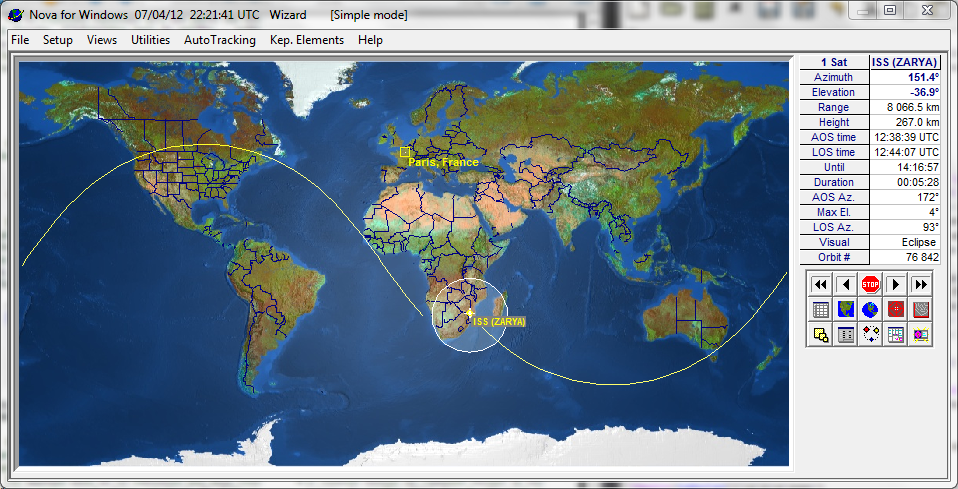
\includegraphics[width=8cm]{pictures/nova3.png}
  \end{center}
\caption{NLSA Nova software}
\label{fig:nlsa_nova}
\end{figure}

\begin{figure}[h]
  \begin{center}
  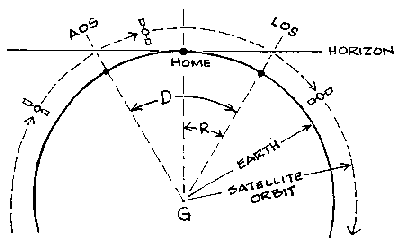
\includegraphics[width=6cm]{pictures/orbitdra.png}
  \end{center}
\caption{Earth orbit representation}
\label{fig:aos_los}
\end{figure}

The antenna rotor will be entirely managed by NLSA Nova software~\cite{nova_um} will send commands through \textsc{rs-232} communication port to the \textsc{gs-232b} (ref ?) micro-controller (wired to the \textsc{gs ?} (ref ?) antenna rotor). This software manages:
\begin {itemize}
\item {orbital elements database and automatic updates from \href{https://www.space-track.org}{Space-Track} ;}
\item {AOS and LOS time information generation ;}
\item {antenna rotor control (\textsc{azimuth} and \textsc{elevation} parameters) following satellite trajectory.}
\end {itemize}

\begin{remark}
  Technical details on the software usage can be found at \textsc{Appendix II}.
\end{remark}

\section {Time-based job scheduling}

\textbf{Method.}
AOS and LOS time information files can be generated by Nova (usual file name \texttt{Nova listing data.TXT}) as specified below:
\begin{enumerate}
\item {Choose the satellite and the observer (\texttt{Configure current view})}
\item {\textup{Utilities} $\rightarrow$ \textup{Listing}}
\item {\textup{One Observer AOS/LOS} $\rightarrow$ \textup{ReCalc}}
\item {\textup{Capture Listing} $\rightarrow$ \textup{ASCII Text File} (Entire listing)}
\end{enumerate}

\begin{remark}
  { \color{rltred}{\Radioactivity} }
  \textsc{(aos/los time information syntax)}
  AOS and LOS time informations returned by Nova are saved in a syntax whose grammar is given in Extended Backus$-$Naur Form (\textsc{ebnf})~\cite{EBNF} (\textsc{figure}~\ref{fig:EBNF_Nova}).
\end{remark}

\begin{remark}
  \textsc{(time zone)}
  For software implementation convenience, we assume the machine time zone is configured at \texttt{UTC} or \texttt{GMT+0}.
\end{remark}

\begin{definition}
  { \color{rltred}{\Radioactivity} }
  \textsc{(acquisition sequence)}
  An \textit{acquisition sequence} is specified by a couple of times which respectively matches with the AOS and the LOS. We denote $\mathcal{S}$ a set of ordered acquisition sequences specification.
\end{definition}

We suggest the following algorithm (\textsc{algorithm}~\ref{algo_timer}, \textsc{implementation~\ref{fig:algo_timer_labview}}) to implement a time-based scheduler for continuous acquisitions from AOS to LOS.

\begin{algorithm}[h]
\caption{Scheduler}
\label{algo_timer}
\begin{algorithmic}[1]
  \REQUIRE non-empty time-ordered $\mathcal{S}$, $t_i()$ : time at call of $t_i$, $F_s$ : file associated to sequence $s$, $F_r$ : refresh rate
  \FOR {$s \in \mathcal{S}$}
  \WHILE {$\lnot (t_d (s) \leq t_i() < t_f (s)) \wedge (t_i() < t_f (s))$}
  \STATE \texttt{sleep}$(\frac{1}{F_r})$ \hfill // \textit{refresh}
  \ENDWHILE
  \STATE $F_s$ $\leftarrow$ \texttt{Logging acquisition loop}($t_i (), t_d (s), t_f (s)$)
  \ENDFOR
  \RETURN $F_{s_1}, \dots, F_{s_{\left | \mathcal{S} \right |}}$
\end{algorithmic}
\end{algorithm}

\begin{figure*}[h]
  \begin{center}
  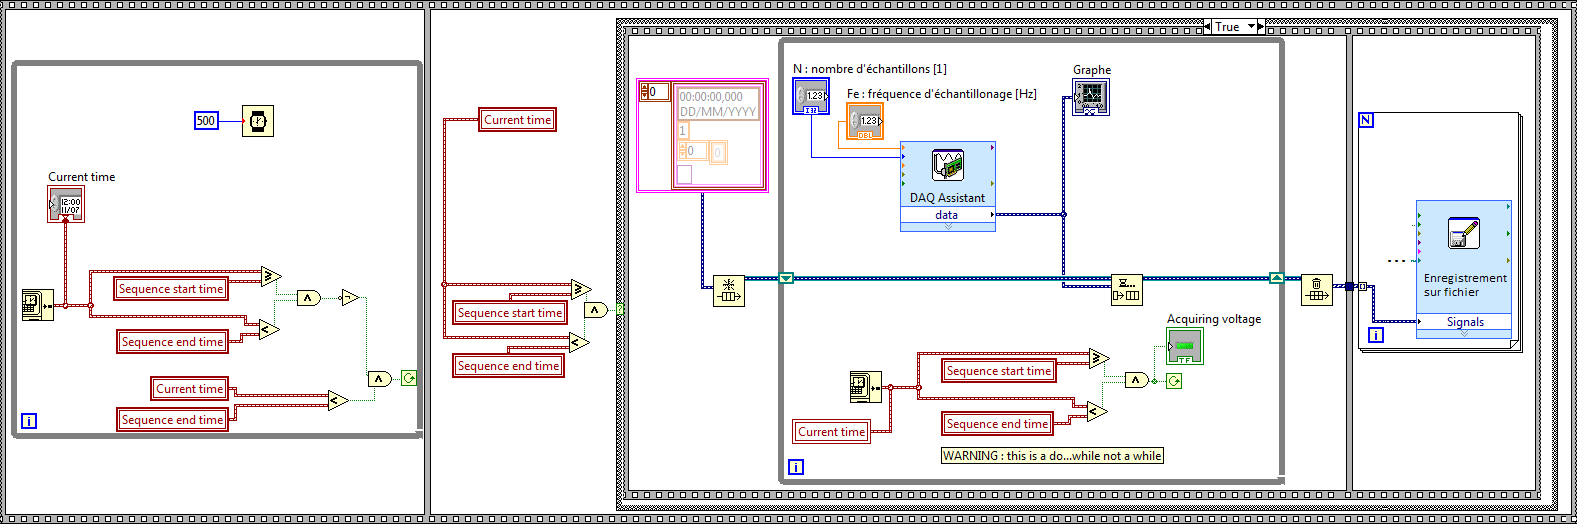
\includegraphics[width=17.5cm]{pictures/minuterie.png}
  \end{center}
\caption{Scheduler implemented in LabVIEW}
\label{fig:algo_timer_labview}
\end{figure*}

\begin{remark}
  \textsc{(accuracy of acquisition sequence release and stop)}
  If we assume $\varepsilon > 0$ we label $F_r$ the scheduler refresh rate. We may have an acquisition start delay of $\frac{1}{F_r} - \varepsilon$. Moreover if we assume the logging acquisition loop is called with $F_e$ and $N$, we may have a acquisition overflow of $\frac{N}{F_e} - \varepsilon$ (acquisition window length).
\end{remark}

\section{Acquisition loop}

\noindent
\textbf{Repository.} A set of tools for acquisition matters are available in the \href{https://github.com/EmptyStackExn/ipgp-pratham-daq-collection}{\texttt{ipgp-pratham-daq-collection}} repository. Final sources are supposed to be compiled with NI Application Builder~\cite{NI_compiler}~\cite{NI_application_builder}.

\begin{definition}
  (\textsc{acquisition window length})
  The \textit{acquisition window length} is the time duration of one acquisition of $N$ samples at a sampling rate of $F_e$ given by the formula
  \begin{eqnarray*}
    \Delta t \overset{\underset{\Delta}{}}{=} \frac{N}{F_e}
  \end{eqnarray*}
\end{definition}

\begin{definition}
  (\textsc{acquisition loop})
  An \textit{acquisition loop} in a loop control structure for repeted and regular acquisitions.
\end{definition}

A sequence of acquisitions is implemented by an acquisition loop (\textsc{algorithm}~\ref{algo_boucle_acquisition}) which calls a set of functions provided by NI-DAQmx libraries~\cite{NI_acquisition_design_ref} with a return type of Dynamic Type~\cite{NI_Dynamic_data}.

%~\cite{MSDN_memory}~\cite{NI_extend_memory}~\cite{NI_deallocation}

\begin{remark}
  Delays between data logging and acquiring function recall are assumed to be handled by the NI LabVIEW API through the usage of \textsc{fifo} memories in the NI USB-6353 Acquisition Box\cite{NI_6353_datasheet}.
\end{remark}

\begin{algorithm}[h]
\caption{Logging acquisition loop}
\label{algo_boucle_acquisition}
\begin{algorithmic}[1]
  \REQUIRE $t_i()$ : initial time, $t_d$ : acquisition start time, $t_f$ : acquisition end time, $F_e$ : sampling rate, $N$ : number of samples a window
  \STATE $F$ : fichier
  \WHILE {$t_d \leq t_i() < t_f$}
  \STATE $F \Leftarrow$ \texttt{acquire}$(F_e, N)$
  \ENDWHILE
  \RETURN $F$
\end{algorithmic}
\end{algorithm}


\section{Frequency component detection}

{ \color{rltred}{\Radioactivity} } This section may be omitted from the understanding of the software system. It is only suggested as a reminder for the use of \textsc{fft}-based \textsc{spectrum analyzers}.

\textbf{Repository.} We provide however an implementation in \textsc{c} of a FFT$-$based sprectum analyzer in the \href{https://github.com/EmptyStackExn/spectra}{\texttt{spectra}} repository.

\begin{definition}
\textsc{(frequency spectrum)}
Let $\mathcal{F}$ be the discrete Fourier transform of an integrable fonction on $\mathbb{R}$ and $\hat{x} = \mathcal{F}(x) = \left [ k \mapsto \hat{x}(k)\right ]$ the \textit{frequency spectrum} of $x$ (at the $k$th sample). We have\cite{Senlis} :
\begin{eqnarray*}
\hat{x}(k) &\overset{\underset{\Delta}{}}{=}& \sum^{N - 1}_{n = 0}{x(n)e^{\frac{-2ik \pi n}{N}}}\\
           &=& \sum^{N - 1}_{n = 0}{x(n)\cos \left ( \frac{2k \pi n}{N} \right )} - i\sum^{N - 1}_{n = 0}{x(n)\sin \left ( \frac{2k \pi n}{N} \right )}
\end{eqnarray*}
\end{definition}

We denote $A (f)$ the amplitude of the frequency component $f$.

\begin{proposition}
\textsc{(amplitude)}
The Fourier transform of a signal of $N$ samples is a map which for an index $k \in \{0 ; N - 1\}$ associates the amplitude of the frequency $f$ such that $f = \frac{k.F_e}{N}$.
\end{proposition}

We then have\cite{Senlis} :
\begin{eqnarray*}
  A (f) &\overset{\underset{\Delta}{}}{=}& \left \| \hat{x} \left (\frac{f.N}{F_e} \right ) \right \|\\
        &=& \sqrt{\mathfrak{Re} \left ( \hat{x} \left (\frac{f.N}{F_e} \right ) \right )^2 + \mathfrak{Im} \left ( \hat{x} \left (\frac{f.N}{F_e} \right ) \right )^2}
\end{eqnarray*}

\section{FM demodulation}

We assume \textsc{fsk} and \textsc{ook} demodulation to be made by the \textsc{vr5000} Transceiver. Retrieving bits of data refers to the \textsc{nrz} decoding section.

\section{NRZ decoding}

\noindent
\textbf{Repository.} The \textsc{nrz} decoder is available in the \href{https://github.com/EmptyStackExn/ipgp-nrz-decoder}{\texttt{ipgp-nrz-decoder}} repository.

\noindent
\textbf{Specification.}
  The digital baseband transmission method is of the kind non-return-to-zero (\textsc{nrz}). In other words, logical \texttt{1} matches with one significant condition and logical \texttt{0} with another.

We assume we have a \textsc{fm} demodulated signal and that we will only focus on shape issue. We suggest different algorithms for same purposes.

\begin{proposition}
  \textsc{(samples per window)}
  We denote $N_w$ as the number of samples per calculation window. Assume one logic bit to be on a time duration $\Delta t = \frac{1}{F_b}$. We have:
  \begin{eqnarray}
    N_w = \frac{F_e}{F_b}
  \end{eqnarray}

  The calculation window length (expressed in number of samples) of the digitizer is $\frac{F_e}{F_b}$.
\end{proposition}

\begin{algorithm}[h]
\caption{NRZ decoder based on mean comparison}
\label{algo_numerisation_FSK}
\begin{algorithmic}[1]
  \REQUIRE signal $x$ \`of $N$ values, amplitude of $f_0$ : $A(f_0)$ and amplitude of $f_1$ : $A(f_1)$
  \STATE $\texttt{mean} \leftarrow \frac{1}{N}\sum^N_{i = 0}{x(i)}$
  \IF {$\left | \texttt{mean} - A(f_0) \right | > \left | \texttt{mean} - A(f_1) \right |$}
  \RETURN \texttt{0}
  \ELSE
  \RETURN \texttt{1}
  \ENDIF
\end{algorithmic}
\end{algorithm}

\section{AX.25 packets decoding}

\textbf{Repository.} The \textsc{ax.25} decoder is available in the \href{https://github.com/EmptyStackExn/ipgp-ax25-decoder}{\texttt{ipgp-ax25-decoder}} repository.

\begin{definition}
  { \color{rltred}{\Radioactivity} }
  \textsc{(lsb$-$msb)}
  Let $x$ be a number in binary representation. There exists a finite sequence $\left ( b_n \right )_{0 \leq n \leq n_0}$ of whole numbers that equals to $0$ or $1$ such that 
  \begin{eqnarray*}
    x = \sum^{n_0}_{n = 0}{b_n \times 2^n}
  \end{eqnarray*}
  The whole number $b_0$ is called the \textit{least significant bit} (\textsc{lsb}) and the number $b_{n_0}$ the \textit{most significant bit} (\textsc{msb}).
\end{definition}

\begin{remark}
  (\textsc{bit endianness})
  Every bytes (words on bits of length $8$) of a \textsc{ax.25} packet (except for the FCS unit) are received with the \textsc{least significant bit} first\cite{IITB}.
\end{remark}

We define the alphabet $\mathbb{B}$ as $\{\texttt{0} ; \texttt{1}\}$ and give the following definition for a standard Pratham AX.25 packet.

\begin{definition}
  \textsc{(ax.25 packet of pratham)}
  A word $m$ on $\mathbb{B}^{\star}$ is an \textsc{ax.25 packet of pratham}~\cite{IITB}~\cite{ax25} if there exists a sequence of the following words (or \textsc{units}) (at one flag at least):

\begin{center}
  \begin{footnotesize}
    \begin{tabular}{|c|c|c|c|c|c|c|}
      \hline
      \multicolumn{7}{|c|}{$m$ : 114 bytes}\\
      \hline
      Flag & Address & Control & PID & {\tiny Information} & FCS & Fanion\\
      \hline
      $\texttt{01111110}$ & $\dots$ & $\texttt{00000011}$ & $\texttt{11110000}$ & $\dots$ & $2$ bytes & $\texttt{01111110}$\\
      \hline
    \end{tabular}
  \end{footnotesize}
\end{center}


\begin{center}
  \begin{footnotesize}
    \begin{tabular}{|c|c|c|c|c|c|c|c|}
      \hline
      \multicolumn{8}{|c|}{Address : 21 octets}\\
      \hline
      \multicolumn{3}{|c|}{Subaddress$_1$} & \multicolumn{2}{c|}{Subaddress$_2$} & \multicolumn{3}{c|}{Subaddress$_3$}\\
      \hline
      \multicolumn{3}{|c|}{7 bytes} & \multicolumn{2}{c|}{7 bytes} & \multicolumn{3}{c|}{7 bytes}\\
      \hline
      \texttt{CQ} & $\left ( (20)_{\operatorname{hex}} \right )^4$ & \texttt{01100000} & \texttt{VU2DMQ} & \texttt{01100000} & \texttt{RELAY} & $(20)_{\operatorname{hex}}$ & \texttt{01100000}\\
      \hline
    \end{tabular}
  \end{footnotesize}
\end{center}

\begin{center}
  \begin{footnotesize}
    \begin{tabular}{|c|}
      \hline
      Information : 87 bytes\\
      \hline
      \textit{Health monitoring data}\cite{IITB}\\
      \hline
    \end{tabular}
  \end{footnotesize}
\end{center}

\end{definition}

The information unit description is defined in \cite{IITB}.


\begin{lemma}
  (\textsc{syntax grammar of AX.25 packet bits})
  The grammar for AX.25 packets given in ~\ref{fig:EBNF_ax25} is linear. Thus, there exists a finite state transducer which parses this grammar.
\end{lemma}

\begin{figure*}
{\scriptsize
\begin{verbatim}
AX.25 packets protocol
--------
packets     ::= { frame }
frame       ::= flag+ address control pid information fcs flag
flag        ::= "01111110"
address     ::= "CQ" ((20)_hex)^4 "01100000" "VU2DMQ" "01100000" "RELAY" (20)_hex "01100000" (* à retranscrire *)
control     ::= "00000011"
pid         ::= "11110000"
information ::= (* pratham *)
fcs         ::= (* attention au boutisme *)
\end{verbatim}
}
\caption{Grammar of Pratham packets en AX.25}
\label{fig:EBNF_ax25}
\end{figure*}

\begin{remark}
  \textsc{(bit stuffing)}
  Bit stuffing coding is able to seperate flags \texttt{01111110} (hexad\'ecimal \texttt{7E}) from real information given in AX.25 packets\cite{IITB}. During data reception, we ignore \texttt{0} at each successive occurence of \texttt{1} after packets seperation operations.
\end{remark}


\begin{implementation}
  (\textsc{algorithme~\ref{algo_decoupage_trames_ax25}})
  { \color{rltred}{\Radioactivity} }
  We use a finite state transducer in order to parse sequences of AX.25 packets.
\end{implementation}





\section{Morse decoding}

\textbf{Repository.} The Morse decoder is available in the \href{https://github.com/EmptyStackExn/ipgp-morse-decoder}{\texttt{ipgp-morse-decoder}} repository.

\textbf{Link.} Simplex (\textsc{ansi} definition)

\vspace{0.3cm}

\textbf{Specification.}
The Morse code specification for the satellite beacon signal is the same as provided by the International Telecommunication Union~\cite{ITU_morse}. We give a short description:

\begin{enumerate}
  \item{The \textsc{dah} letter ($-$) lasts three times longer than the \textsc{dit} letter ($\cdot$) ;}
  \item{L'\'ecart entre deux \'el\'ements (\textsc{dit} ou \textsc{dah}) d'une m\^eme lettre dure un \textsc{dit} ;}
  \item{L'\'ecart entre deux lettres d'alphabet dure un \textsc{dah} ;}
  \item{L'\'ecart entre deux mots dure sept \textsc{dit}.}
\end{enumerate}

\begin{definition}
  We denote $\mathbb{B}$ as the set of bits, $\mathbb{M}$ the Morse alphabet and $\mathbb{N}_{255}$ the ASCII representable characters as follows:
  \begin{eqnarray*}
    \mathbb{B}      &=& \left \{ \texttt{0} ; \texttt{1} \right \}\\
    \mathbb{M}      &=& \left \{ \varepsilon_1, \varepsilon_3, \varepsilon_7, ., - \right \}\\
    \mathbb{N}_{255} &=& \left \{ \dots ; \textup{a} ; \textup{b} ; \dots \right \}
  \end{eqnarray*}
\end{definition}

\begin{definition}
  We define on $\mathbb{M}$ the coding function for one token (??? inexact):
  \begin{eqnarray*}
    \operatorname{morse\_code} : \mathbb{M} &\rightarrow& \mathbb{B^{*}}\\
                 m &\mapsto&
                 \left\{\begin{matrix}
                        \texttt{0} \ &\textup{if}& \ m &=& \varepsilon_1 \\ 
                        \texttt{000} \ &\textup{if}& \ m &=& \varepsilon_3 \\
                        \texttt{0000000} \ &\textup{if}& \ m &=& \varepsilon_7 \\
                        \texttt{1} \ &\textup{if}& m &=& \cdot\\
                        \texttt{111} \ &\textup{if}& m &=& -
                        \end{matrix}\right.
  \end{eqnarray*}
\end{definition}

\begin{definition}
  We define on $\mathbb{M}$ the length of a letter $x \in \mathbb{M}$ as:
\begin{eqnarray*}
  L : \mathbb{M} &\rightarrow& \mathbb{N}\\
              x  &\mapsto&
                 \left\{\begin{matrix}
                 1 \ &\textup{if }& x &\in& \left \{ \texttt{.}, \varepsilon_1 \right \} \\
                 3 \ &\textup{if }& x &\in& \left \{ -, \varepsilon_3 \right \} \\ 
                 7 \ &\textup{if }& x &=& \varepsilon_7
              \end{matrix}\right.
\end{eqnarray*}
\end{definition}

\begin{figure*}[]
  \begin{eqnarray*}
    \underbrace{\underbrace{\underbrace{\texttt{1}}_{.} \underbrace{\texttt{0}}_{\varepsilon_1} \underbrace{\texttt{1}}_{.}}_{I} \underbrace{\texttt{000}}_{\varepsilon_3} \underbrace{\underbrace{\texttt{1}}_{.} \underbrace{\texttt{0}}_{\varepsilon_1} \underbrace{\texttt{1}}_{.}}_{I} \underbrace{\texttt{000}}_{\varepsilon_3} \underbrace{\underbrace{\texttt{111}}_{-}}_{T}}_{IIT}
    \underbrace{\texttt{1111111}}_{\varepsilon_7}
    \underbrace{\underbrace{\underbrace{\texttt{111}}_{-} \underbrace{\texttt{0}}_{\varepsilon_1} \underbrace{\texttt{1}}_{.} \underbrace{\texttt{0}}_{\varepsilon_1} \underbrace{\texttt{1}}_{.} \underbrace{\texttt{0}}_{\varepsilon_1} \underbrace{\texttt{1}}_{.}}_{B} \underbrace{\texttt{000}}_{\varepsilon_3} \underbrace{\underbrace{\texttt{111}}_{-} \underbrace{\texttt{0}}_{\varepsilon_1} \underbrace{\texttt{111}}_{-} \underbrace{\texttt{0}}_{\varepsilon_1} \underbrace{\texttt{111}}_{-}}_{O} \underbrace{\texttt{000}}_{\varepsilon_3} \underbrace{\underbrace{\texttt{111}}_{-} \underbrace{\texttt{0}}_{\varepsilon_1} \underbrace{\texttt{111}}_{-}}_{M}}_{BOM}
  \end{eqnarray*}  
  \caption{Example of token generation steps for the Morse coded beacon signal : ``\texttt{IIT Bombay}''}
  \label{fig:exemple_signal_morse}
\end{figure*}


\begin{figure}[h]
  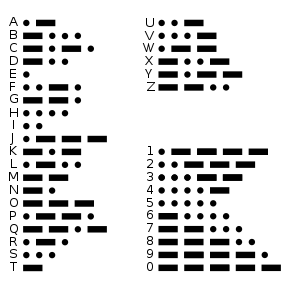
\includegraphics[width=6cm]{pictures/morse.png}
\caption{Morse code alphabet}
\label{fig:morse}
\end{figure}

\textbf{Implementation.} We implement a transducer with two entrypoints (or two transducers with one unique entrypoint) with a lexical analyzer generator from the alphabet $\mathbb{B}^{\star} = \{ \texttt{0} ; \texttt{1} \}^{\star}$ to $\mathbb{M}^{\star}$. The second transducer processes from $\mathbb{M}^{\star}$ to $\mathbb{N}_{255}^{\star}$ (\textsc{figure} ~\ref{fig:transducteur_morse}).

\begin{figure*}
  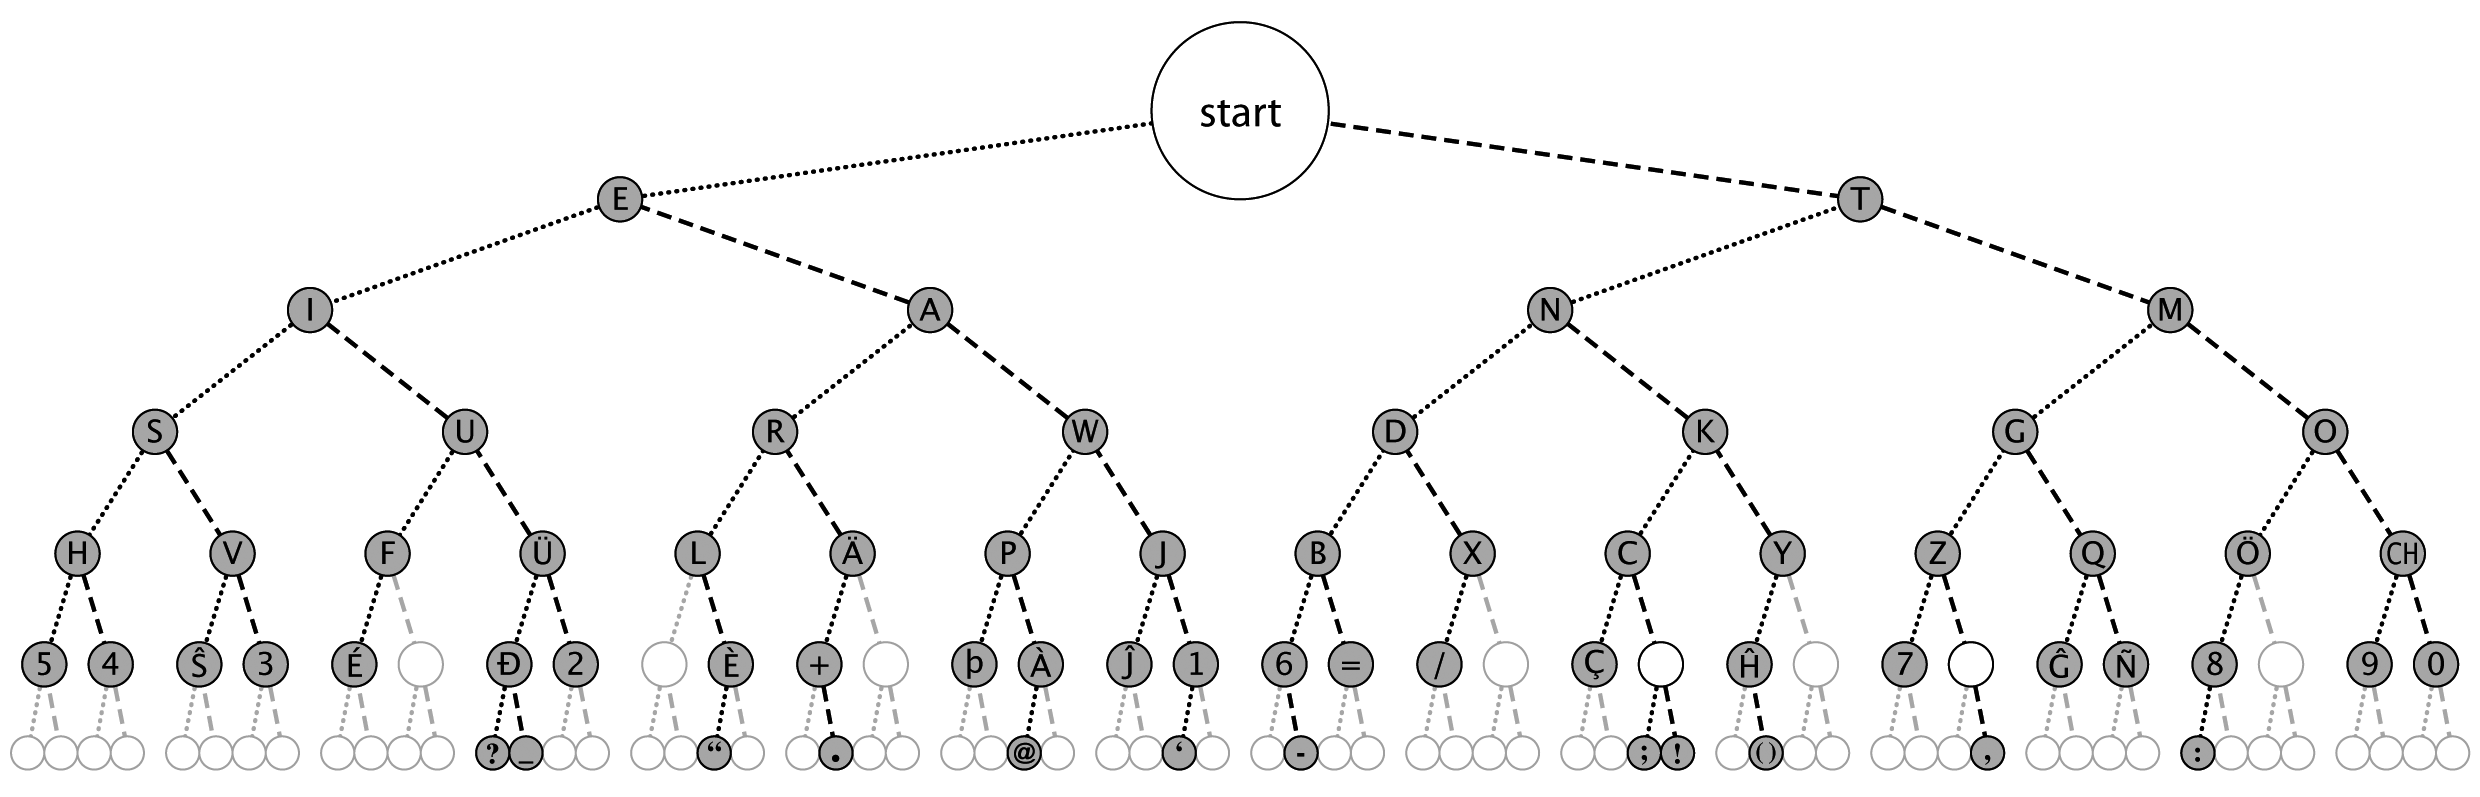
\includegraphics[width=17cm]{pictures/Morse_code_tree3.png}
\caption{Transducteur fini associ\'e au d\'ecodage \textsc{morse}~\cite{copyright_transducteur_morse}}
\label{fig:transducteur_morse}
\end{figure*}

\section{Data logging}

We remind that data logging rules are specified in \textit{Pratham satellite : File format specification document}\cite{IITB_filespec}. Duration of satellite AOS depends on the following parameters:

\begin{itemize}
\item{the satellite altitude ;}
\item{the Earth orbit model used in the tracking softwware ;}
\item{the antenna aperture (???) ;}
\item{the low elevation multi-targeting (???)}
\end{itemize}

We give a preliminary estimation of total logging file sizes considering that a measure may be represented in decimal ASCII character representation with 6 digits.

\begin{proposition}
  (\textsc{space complexity of a floating-point number})
  Assuming that a floating-point number will be represented on $6$ digits and that an encoding character costs $1$ byte. A floating-point number then costs $7$ bytes.
\end{proposition}

\begin{remark}
  A floating-point number represented in IEEE ??? on $32$ bits only costs $4$ bytes $-$ that is to say threes times cheaper that the previous representation $-$
\end{remark}

\begin{proposition}
  (\textsc{space complexity of Data 0- Calibration info, station characteristics})
  Let $(\mathbb{B}^{\star}, l_{\cdot})$ be a normed space (???). We then have the following approximation for one acquisition sequence:
\end{proposition}

\begin{proposition}
  (\textsc{space complexity of Data 1- Raw output from ground station acquisition})
  Let $(\mathbb{B}^{\star}, l_{\cdot})$ be a normed space (???). We then have the following approximation for one acquisition sequence:
\end{proposition}

\begin{proposition}
  (\textsc{space complexity of Data 2- Orientation of the reference})
  Let $(\mathbb{B}^{\star}, l_{\cdot})$ be a normed space (???). We then have the following approximation for one acquisition sequence:
\end{proposition}

\begin{proposition}
  (\textsc{space complexity of Data 3- Auxiliary data})
  Let $(\mathbb{B}^{\star}, l_{\cdot})$ be a normed space (???). We then have the following approximation for one acquisition sequence:
\end{proposition}

\begin{proposition}
  (\textsc{space complexity of Data 4- Processed data})
  Let $(\mathbb{B}^{\star}, l_{\cdot})$ be a normed space (???). We then have the following approximation for one acquisition sequence:
\end{proposition}

\begin{proposition}
  (\textsc{space complexity of Data 4- Processed data})
  Let $(\mathbb{B}^{\star}, l_{\cdot})$ be a normed space (???). We then have the following approximation for one acquisition sequence:
\end{proposition}

\begin{proposition}
  (\textsc{space complexity of Data 5- Processed data for Prathart})
  Let $(\mathbb{B}^{\star}, l_{\cdot})$ be a normed space (???). We then have the following approximation for one acquisition sequence:
\end{proposition}


  \begin{eqnarray}
    l_{\textup{file}} &=& \underbrace{\Delta t}_{\in \left [ 7 ; 13 \right ] \ \operatorname{min}} \times \underbrace{f_e}_{10 \ \operatorname{kHz}} \nonumber\\
                    &\times& \underbrace{\left (\underbrace{l_{\textup{date}}}_{23 \ \operatorname{octets}} + \underbrace{n_{\textup{voies}}}_{12} \times (\underbrace{l_{\textup{flottant}}}_{12 \ \operatorname{octets}} + \underbrace{l_{\textup{separateur}}}_{1 \ \operatorname{octet}} ) \right )}_{\textup{une ligne}}\\
                    &\in& \left [ 7,518 \times 10^8 ; 1,3962 \times 10^9 \right ] \\
                    &\ &  \textup{as } \Delta t \mapsto l_{\textup{fichier}} (\Delta t) \ \textup{increases} \nonumber
  \end{eqnarray}

Considering a estimation model for the number of satellite AOS over Paris\cite{IPGP_simul_loic} :
\begin{eqnarray}
  n_{\textup{AOS/day}} \in \left [ 4 ; 6 \right ] \ \textup{AOS}
\end{eqnarray}

We then have, per day :

\begin{eqnarray}
  l_{\textup{jour}} &=& n_{\textup{passages/jour}} \times l_{\textup{fichier}}\\
                &\in& \left [ 3,0072 \times 10^9 ; 8,3772 \times 10^9 \right ] \\
                &\ & \textup{car } n_{\textup{passages/jour}} \mapsto l_{\textup{jour}} (n_{\textup{passages/jour}}) \ \textup{croissante} \nonumber
\end{eqnarray}

Sur un fonctionnement suppos\'e de 4 mois\cite{IITB_general} du satellite, il est n\'ecessaire de disposer d'un espace de stockage d'au moins :

\begin{eqnarray}
  l_{\textup{total}} &=& n_{\textup{passages/jour}} \times 30,5 \times 4 \times l_{\textup{fichier}}\\
                 &\in& \left [ 3,668784 \times 10^{11} ; 1,0220184 \times 10^{12} \right ]
\end{eqnarray}



On pr\'esente en \textsc{table}~\ref{tab:estimations_stockage}, les estimations de taille de fichier concernant les donn\'ees brutes à la sortie de l'acquisition.

\begin{table}[h]
  \caption{Estimations minimales et maximales de l'espace de stockage n\'ecessaire aux donn\'ees brutes}
  \begin{center}
    \begin{tabular}{@{\hspace{9pt}} c @{\hspace{9pt}} ||
        @{\hspace{6pt}} c @{\hspace{6pt}} | @{\hspace{6pt}} c
       @{\hspace{6pt}} }
      
      \hline\hline
      \multirow{2}{*}{Dur\'ee de temps (s)} & \multicolumn{2}{c}{Taille des fichiers {\hspace{9pt}} } \\
                                            & \textsc{min} & \textsc{max} \\ \hline
                                      1 min & \multicolumn{2}{c}{$107,4$ Mo} \\
                              1 seq. d'acq. & $751,8$ Mo & $1,4$ Go \\
                                     1 jour & $3,0$ Go & $8,37$ Go \\
                                     1 mois & $91,7$ Go & $255,5$ Go \\
                                     4 mois & $366,8$ Go & $1,02$ To \\
      \hline\hline

    \end{tabular}
  \end{center}
  \label{tab:estimations_stockage}
\end{table}

En consid\'erant que la fr\'equence d'\'echantillonage $F_e$ est de $10$ kHz, on obtient un instant de mesure
\begin{eqnarray*}
  T_e \stackrel{\Delta}{=} \frac{1}{F_e}
\end{eqnarray*}

Par passage de satellite, on n'obtient que 7200000 valeurs pour les slanTEC (calcul \`a justifier).

Dans le cadre d'une solution provisoire, on se permet d'utiliser le format de fichier de ``LabVIEW Measurement File''~\cite{NI_lvm} (\underline{solution \`a probleme car enregistre avec la date d'enregistrement et non la date d'acquisition}).

\chapter{File formats}
\label{sec:file_formats}

\section{Nova AOS/LOS timestamps file format}

We give in EBNF the syntax grammar for AOS and LOS information returned by Nova. We show that a part of this grammar is linear. Thus, the formed language is regular and there exists a regular expression which denotes it. We then parse a file using the \texttt{Scan From String}~\cite{NI_scan_from_string} function. 


\begin{figure*}[h]
{\scriptsize
\begin{verbatim}
Nova satellite AOS/LOS file
--------
file         ::= columns_desc { day_eclipses }

columns_desc ::= "Date (Z)" "AOS (Z)" "LOS (Z)" "Duration" "Between Az" '@' "AOS Max El Az" '@' "LOS Height" "km" newline

day_eclipses ::= day_header { day_entry }
day_header   ::= { character } "at" { character } ',' { character } newline
day_entry    ::= date time time time time int_number '°' int_number '°' int_number '°' float_number newline

date         ::= int_number '/' int_number '/' int_number
time         ::= int_number ':' int_number ':' int_number

newline      ::= \n
character    ::= 'a'|'b'|..|'A'|'B'|..|'0'|'1'|..
int_number   ::= [ '-' | '+' ] { '0' | .. | '9' }
float_number ::= [ '-' | '+' ] { '0' | ... | '9' } '.' { '0' | ... | '9' }
\end{verbatim}
}
\caption{Grammar of AOS/LOS information returned by Nova}
\label{fig:EBNF_Nova}
\end{figure*}

\begin{lemma}
  The restriction of ~\ref{fig:EBNF_Nova} whose start symbol is \texttt{day\_eclipses} is a linear grammar.
\end{lemma}

\begin{figure*}[h]
  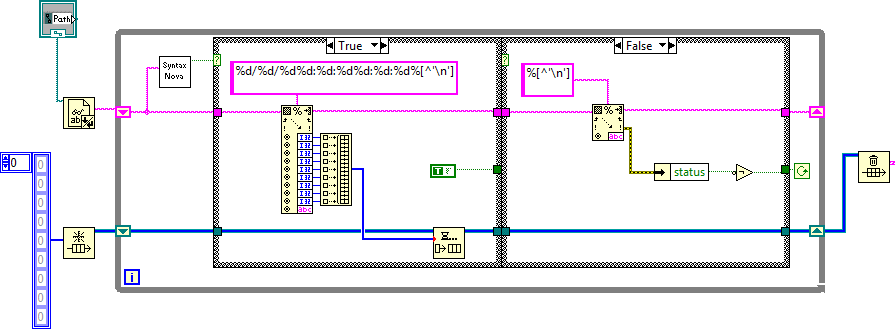
\includegraphics[width=17cm]{pictures/parser_nova_labview.png}
  \caption{Regular expression which denotes the restriction whose start symbol is \texttt{day\_eclipses}}
\label{fig:algo_scan_parse_nova_labview}
\end{figure*}

\begin{lemma}
  There exists a regular expression which denotes the language formed by the restriction of ~\ref{fig:EBNF_Nova} and is given in \ref{fig:algo_scan_parse_nova_labview}.
\end{lemma}








\section{Pratham data log}
Pratham file formats decided betwwen IPGP and IITB for vertical and slant TEC are specified in ??? whose we give a syntax grammar in EBNF in ~\ref{fig:syntaxe_Pratham_format}.

\begin{figure*}[h]
{\scriptsize
\begin{verbatim}
Raw output file from ground station acquisition (RAW_PRAT_SSSS_yyyy_ddd_hh_mm_ss.txt)
-------------------------
file ::= "Station_ID"             word
         "Location"               int_number ':' int_number ':' float_number int_number ':' int_number ':' float_number int_number
         "Satellite_Tracking_ID"  word
         "Start_time_UT"          time_stamp
         "End_time_UT"            time_stamp
         "Sampling_rate"          int_number
         "Data_points"            float_number
         "Acquisition_type"       int_number
         "Time" "145_VMAG1" "145_VPHS1" "145_VMAG2" "145_VPHS2" "437_VMAG1" "437_VPHS1" "437_VMAG2" "437_VPHS2"
         { time_stamp float_number float_number float_number float_number float_number float_number float_number float_number }

time_stamp   ::= int_number ':' int_number ':' int_number ':' int_number ':' int_number

word         ::= { character }
character    ::= 'a' | 'b' | ... | 'z' | 'A' | 'B' | ... | 'Z' | '0' | '1' | ... | '9'
int_number   ::= [ '-' | '+' ] { '0' | ... | '9' }
float_number ::= [ '-' | '+' ] { '0' | ... | '9' } '.' { '0' | ... | '9' }

\end{verbatim}
}
  \caption{Pratham raw data logs grammar}
  \label{fig:syntaxe_Pratham_format}
\end{figure*}

\begin{proposition}
  The grammar \ref{fig:syntaxe_Pratham_format} is linear and forms a regular language.
\end{proposition}


\chapter{Measurement and computation accuracy}
\label{sec:results}

\section {Earth orbit model}

The Earth orbit model chosen is \textsc{sgp4/sdp4} model.

\section{Measurement accuracy}

The ADC has a resolution of $16$ bits. We denote $Q$ as the \textsc{resolution} or \textsc{least significant bit voltage} (in volts). The maximum error that the instrument gives under the usual conditions are given by the ADC specifications (Section \textit{AI Absolute Accuracy Table}, p.5)~\cite{NI_6353_datasheet} and are confirmed by the following calculation for a \textsc{span} of $20 \operatorname{V}$:
\begin{eqnarray*}
  Q &=& \frac{E_{\textup{FSR}}}{N}\\
    &=& \frac{V_{\textup{RefHi}} - V_{\textup{RefLow}}}{2^M - 1}\\
    &=& \frac{10 - (-10)}{2^{16} - 1}\\
    &\simeq& 0.0001520 \operatorname{V}
\end{eqnarray*}

where :

\begin{description}
  \item[$E_{\textup{FSR}}$]{ : full scale voltage range (V)}
  \item[$N$]{ : number of voltage intervals [1]}
  \item[$V_{\textup{RefHi}}$]{ : upper extreme coding voltage (V)}
  \item[$V_{\textup{RefLow}}$]{ : lower extreme coding voltage (V)}
  \item[$M$]{ : ADC resolution (bits)}
\end{description}

Considering that $V_{\textup{RefHi}} = 10 \operatorname{V}$, for all acquired voltage $U_a$, $U_a$ will be expressed in scientific notation as follows:
\begin{eqnarray*}
  U_a = \left ( d_1.d_2d_3d_4d_5d_6d_7d_8 \pm 0.0001520 \right ) \operatorname{V}
\end{eqnarray*}

We then decide to keep $8$ digits for a voltage measured with this ADC. However, further calculations have to be based on the number of \textsc{significant digits} which is $6$. 

\section{Sampling}
We suggest to introduce some denotations for further configurations.

\begin{notation}
  Let $x$ be a discrete signal of $N$ samples indexed by a set $I$ in the form $x : I \rightarrow \mathbb{R}, t \mapsto x(t)$. We denote the following physical quantities
  \begin{description}
  \item[$F_c$]{ : central frequency [Hz]}
  \item[$\Delta f$]{ : bandwidth length [Hz]}
  \item[$F_e$]{ : sampling rate [Hz]}
  \item[$F_b$]{ : bit rate of the modulated signal [Hz = $\operatorname{bits}.\operatorname{s}^{-1}$]}
  \item[$N$]{ : number of samples [1]}
  \item[$\Delta t$]{ : acquisition window length [s]}
  \end{description}
\end{notation}

\noindent
\textbf{Configuration.} The usage of \texttt{DAQ Assistant} function is deprecated but still remains possible with the following configuration:
\begin{itemize}
  \item{\texttt{Acquisition mode} : choose \texttt{Continuous Samples}}~\cite{NI_continuous_samp}
  \item{\texttt{Samples to Read} : $N$}
  \item{\texttt{Rate (Hz)} : $F_e$}
\end{itemize}

\begin{remark}
  (\textsc{fifo memory})
  The NI USB-6353 Acquisition Box has a \textsc{fifo} memory size of $4095$ samples~\cite{NI_6353_datasheet}.
\end{remark}

\begin{remark}
  \textsc{(complexity)}
  Le co\^ut en temps de la fonction \texttt{DAQ Assistant} s'exprime en $\Omega(N)$\cite{omega} et prend un temps $\Delta t = \frac{N}{F_e}$ entre l'appel de fonction et le retour des valeurs.
\end{remark}

Signal post-processing allows us to choose a specific \textsc{window length} for further digitizing. For a signal of bit rate $F_b$ the window length is defined as
\begin{eqnarray*}
  \frac{1}{F_b}
\end{eqnarray*}

Assuming the \textsc{fm} demodulation process done by the transceiver, the sampling rate can be focused only on the bit rates in the signal.
\begin{theorem} (\textsc{Nyquist-Shannon}~\cite{Nyquist}~\cite{Shannon})
  \begin{eqnarray}
    F_e \geq 2 \times \operatorname{max} \left \{ F_{b_1} ; F_{b_2} \right \}
  \end{eqnarray}
\end{theorem}

\begin{remark}
  \textsc{(optimal sampling)}
  The previous theorem suggests that - for a digital signal - the base theoretical acquisition frequency is $0,5$ Hz per baud. In fact, we would need at least between $0,7$ and $0,8$ Hz per baud\cite{FV}.
\end{remark}

The \textsc{ni usb-6353} Acquisition Box on multi-channel is able to deliver a maximum sampling rate (aggregate) on multi-channel~\cite{NI_6353_datasheet} of
\begin{eqnarray*}
  F_{e_{\text{MAX}}} &=& 1.00 \text{ MS.s$^{-1}$}\\
                &=& 1.00 \times 10^6 \text{ Hz}
\end{eqnarray*}

Considering that the acquisition will be done simultaneously, it is trivial that all channels have a sampling rate of $2 \times 2,4 \times 10^3 = 4,8 \times 10^3$ Hz (see previous theorem). We may notice however that other \textsc{dsp}s have a limit of $4 \times F_c$ due to computation overflow~\cite{TI_MSP430}.

Finally using a sample rate of $10$ kHz is the most convenient choice we made.


\chapter{Hardware used at IPGP}

\section{Measurement machine}

Les logiciels suivants doivent \^etre install\'es et \'eventullement correctement configur\'es dans l'ordre\cite{NI_driver} suivant:
\begin{enumerate}
  \item{\href{http://digital.ni.com/src.nsf/websearch/968B3DF8AD48394D86257880005141A8?OpenDocument&node=node=203014_us}{LabVIEW 8.6 (National Instruments)}}
  \item{\href{http://joule.ni.com/nidu/cds/view/p/id/2260/lang/fr}{NI DAQ-mx 9.2.3 (pilote du bo\^itier d'acquisition)}}
  \item{\href{http://www.nlsa.com/uploads/nfw21v/nova_21v_download.html}{Nova for Windows 2.2c (NLSA)}}
  \item{\href{http://protz.github.com/ocaml-installer/}{OCaml 3.12 pour Windows}}
\end{enumerate}

Il sera pr\'evu que la machine d'acquisition $-$ pr\'evue pour fonctionner 24h/24 durant 4 mois $-$ sera de type :
\begin{itemize}
  \item{Mod\`ele : \href{http://support.dell.com/support/edocs/systems/latd630a/en/sm/index.htm}{Dell Latitude ATG D630}}
  \item{Processeur : \href{http://ark.intel.com/products/29761/Intel-Core2-Duo-Processor-T7500-\%284M-Cache-2_20-GHz-800-MHz-FSB\%29}{Intel Core 2 Duo T7500 (2,2 GHz, 2,19 GHz)}}
  \item{Syst\`eme d'exploitation : Microsoft Windows XP}
  \item{Disque dur : \href{http://storage.toshiba.com/storagesolutions/archived-models/mk8046gsx}{Toshiba MK8046GSX} (74,3 Go dont 71,5 Go occup\'es) (rapidit\'e d'\'ecriture ?)}
  \item{Carte r\'eseau :
    \begin{itemize}
      \item{LAN: \href{http://www.broadcom.com/support/ethernet_nic/netlink_k57.php}{Broadcom NetXtreme 57xx Gigabit Controller}}
      \item{Wifi: \href{http://www.intel.com/products/wireless/prowireless_mobile.htm}{Intel PRO/Wireless 3945 ABG Network Connection}}
    \end{itemize}
  }
\end{itemize}

Elle sera constemment connect\'ee sur le r\'eseau afin de permettre \`a l'\'equipe de surveiller et de rapatrier les donn\'ees acquises.

\section{Monitoring issues}

\subsection{Rotating antenna}

Skype...

\subsection{Desktop remote control}

\begin{thebibliography}{99}

\bibitem{cecill}Commissariat \'a l'Energie Atomique, Centre National de la Recherche Scientifique, Institut National de Recherche en Informatique et en Automatique, {\it \href{http://www.cecill.info/licences/Licence_CeCILL_V2-en.html}{CeCILL Free Software License Agreement}} (September, 2006)

\bibitem{IITB_general}Saptarshi Bandyopadhyay, Jhonny Jha, Haripriya, Ameya Damle, Deepika Thakur, Sanyam Mulay, Prashant Sachdeva, Jaideep Joshi, Vaibhav Unhelkar, Yashovardhan Chati, Mayank Chaturvedi, Niranjan Parab, Manas Rachh, Shashank Tamaskar, Mallesh Bommanahal, Ashish Goel, Kartavya Neema, Subhasis Das, Vishnu Sresht, Ramnath Pai, Ankit Chiplunkar, {\it \href{http://www.aero.iitb.ac.in/pratham/otherdocs/IIT-B_Paper_Pratham_20thApr.pdf}{Introduction to Pratham, IIT Bombay’s Student Satellite Project}} (IIT Bombay, June 2010)

\bibitem{IITB}J. Jha, S. Bandyopadhyay, C. Talnikar, {\it Pratham - Telemetry and Telecommand Document} (IIT Bombay, November 2010)

\bibitem{IITB_filespec}H. Nguyen Van, P. Co\"isson, P. Godbole, J. Jha, {\it Pratham satellite : File Formats Specification} (IPGP, May 2011)

\bibitem{IPGP_simul_loic}L. Viens, P. Co\"isson, {\it Pratham satellite : Paris Ground Station Simulations} (IPGP, November 2010)

\bibitem{Senlis}J. Senlis, {\it \href{http://jgsenlis.free.fr/dsp_28335.htm}{Formation DSP sur 320F28335}} (INSSET, Universit\'e de Picardie, 2008)

\bibitem{CHLS}T. Capitaine, M. Hamzaoui, A. Lorthois, J. Senlis, {\it \href{http://jgsenlis.free.fr/ax25/Cetsis2008_AX25.pdf}{D\'emodulation et d\'ecodage de trames AX.25 par DSPIC pour la localisation d'un ballon sonde m\'et\'eo dans le cadre d'une action ``Plan\`ete Sciences''}} (CETSIS, Bruxelles, 2008)

\bibitem{ax25}William A. Beech, Douglas E. Nielsen, Jack Taylor, {\it \href{http://www.tapr.org/pdf/AX25.2.2.pdf}{AX.25 Link Access Protocol for Amateur Packet Radio, version 2.2}} (Tucson Amateur Packet Radio Corporation, July 2008)

\bibitem{nova_um}Michael R. Owen, {\it \href{http://www.nlsa.com/docs/nfwdoc.pdf}{Nova for Windows $-$ User's Manual}} (Northern Lights Software Associates, February 2000)

\bibitem{Hoare}C. A. R. Hoare, {\it \href{http://www.spatial.maine.edu/~worboys/processes/hoare%20axiomatic.pdf}{An axiomatic basis for computer programming}} (Communications of the ACM 12 (10): 576-580)

\bibitem{FV}Agn\`es Foucher, Christian Valade, {\it \href{http://radiomods.free.fr/r2000-info/mod_dem_fsk.pdf}{Modulation, D\'emodulation, FSK. \'Etude structurelle}} (Universit\'e de Toulouse 1, F\'evrier 1999)

\bibitem{EBNF}International Organization for Standardization, {\it \href{http://standards.iso.org/ittf/PubliclyAvailableStandards/s026153_ISO_IEC_14977_1996(E).zip}{Information technology $-$ Syntactic metalanguage $-$ Extended BNF}} (ISO/IEC 141977, December 1996)

\bibitem{ITU_morse}International Telecommunication Union, {\it \href{http://www.itu.int/rec/R-REC-M.1677-1-200910-I/}{International Morse code $-$ Recommendation ITU-R M.1677-1}} (ITU, 2009)

\bibitem{NI_driver}National Instruments, {\it \href{http://www.ni.com/gettingstarted/installsoftware/dataacquisition.htm}{Install NI LabVIEW and NI-DAQmx Driver}} (2010)

\bibitem{NI_calibration_procedure}National Instruments, {\it \href{http://www.ni.com/pdf/manuals/370937k.pdf}{B/E/M/S/X Series Calibration Procedure}} (370937K-01, August 2010)

\bibitem{NI_6353_datasheet}National Instruments, {\it \href{http://www.ni.com/pdf/manuals/370787b.pdf}{NI 6351/6353 Specifications}} (370787B-01, August 2010)

\bibitem{NI_DAQ_Assistant}National Instruments, {\it \href{http://zone.ni.com/reference/en-XX/help/371361D-01/lvmeasconcepts/creating_daq_app/}{Creating a Typical DAQ Application}} (371361D-01, August 2007)

\bibitem{NI_acquisition_design_ref}National Instruments, {\it \href{http://zone.ni.com/devzone/cda/tut/p/id/11805}{Data Acquisition Reference Design for LabVIEW}} (July 2010)

\bibitem{NI_continuous_samp}National Instruments, {\it \href{http://digital.ni.com/public.nsf/allkb/B86AA2D2FDE9A16086256FFC00604202}{When Should I Use Continuous or Finite Sampling Modes?}} (3L8BGMXL, May 2005)

\bibitem{NI_extend_memory}National Instruments, {\it \href{http://zone.ni.com/reference/en-XX/help/371361D-01/lvhowto/enable_lrg_ad_aware/}{Extending Virtual Memory Usage for 32-bit Windows}} (371361D-01, August 2007)

\bibitem{NI_deallocation}National Instruments, {\it \href{http://zone.ni.com/reference/en-XX/help/371361D-01/glang/request_dealloc/}{Request Deallocation}} (371361D-01, August 2007)

\bibitem{NI_scan_from_string}National Instruments, {\it \href{http://zone.ni.com/reference/en-XX/help/371361D-01/glang/scan_from_string/}{Scan From String}} (371361D-01, August 2007)

\bibitem{NI_Dynamic_data}National Instruments, {\it \href{http://zone.ni.com/reference/en-XX/help/371361D-01/lvconcepts/expressvis/}{Express VIs, Dynamic Data Type}} (371361D-01, August 2007)

\bibitem{NI_lvm}National Instruments, {\it \href{http://zone.ni.com/devzone/cda/tut/p/id/4139}{Specification for the LabVIEW Measurement File (.lvm)}} (July 2010)

\bibitem{NI_compiler}National Instruments, {\it \href{http://zone.ni.com/devzone/cda/tut/p/id/11472}{NI LabVIEW Compiler: Under the Hood}} (July 2010)

\bibitem{NI_application_builder}National Instruments, {\it \href{http://zone.ni.com/devzone/cda/tut/p/id/4039}{Creating Executables with the LabVIEW Application Builder}} (March 2010)

\bibitem{TI_MSP430}Texas Instruments, {\it \href{http://www.ti.com/lit/an/slaa037/slaa037.pdf}{FSK Modulation and Demodulation With the MSP430 Microcontroller}} (SLAA037, December 1998)

\bibitem{MSDN_memory}Windows Developer Center, {\it \href{http://msdn.microsoft.com/en-us/library/aa366778(VS.85).aspx}{Memory Limits for Windows Releases}} (Microsoft Developer Network, 2009)

\bibitem{Knuth}Donald Knuth, {\it \href{http://books.google.fr/books?id=MooMkK6ERuYC}{The Art of Computer Programming, Volume 1: Fundamental Algorithms, Third Edition}}, Section 2.2.1: Stacks, Queues, and Deques, pp. 238$-$243. (Addison-Wesley, 1997)

\bibitem{ocaml_parsing}Xavier Leroy, Damien Doligez, Alain Frisch, Jacques Garrigue, Didier R\'emy and J\'er\^ome Vouillon, {\it  The OCaml system, release 3.12}, \href{http://caml.inria.fr/pub/docs/manual-ocaml/manual026.html}{Chapter 12: Lexer and parser generators (ocamllex, ocamlyacc)} (INRIA, 2011)

\bibitem{Alexandridis}``{\it A microprocessor with a ``wordlength equal to $n$'' is also referred to as an $n$-bit microprocessor defined as a processor with $n$-bit wide internal data registers and $n$-bit wide ALU (arithmetic logic unit) which carries out operations on $n$-bit input operands.''}, N. Alexandridis in {\it \href{http://www.student.seas.gwu.edu/~kallitec/ece201/TextbookFigures/000-Chapter1.pdf}{Computer Systems Architecture: Microprocessor-Based Designs}} (The George Washigton University, May 1999)

\bibitem{Sannibale}Virg\'inio de Oliveira Sannibale, {\it \href{http://www.ligo.caltech.edu/~vsanni/ph3/SignificantFiguresAndMeasurements/SignificantFiguresAndMeasurements.pdf}{Measurements and Significant Figures}} (California Institute of Technology, October 2011)

\bibitem{Nyquist}H. Nyquist, {\it \href{http://replay.web.archive.org/20060706192816/http://www.loe.ee.upatras.gr/Comes/Notes/Nyquist.pdf}{Certain topics in telegraph transmission theory}}, Trans. AIEE, vol. 47, pp. 617–644, Apr. 1928. Reprint as classic paper in: Proc. IEEE, Vol. 90, No. 2, Feb 2002.

\bibitem{Shannon}C. E. Shannon, {\it \href{http://www.stanford.edu/class/ee104/shannonpaper.pdf}{Communication in the presence of noise}}, Proc. Institute of Radio Engineers, vol. 37, no.1, pp. 10–21, Jan. 1949. Reprint as classic paper in: Proc. IEEE, Vol. 86, No. 2, (Feb 1998).

\bibitem{Comment1} Jhonny Jha : ``f0 would mean 1 and f1 would mean 0 is what I intended to say''

\bibitem{omega} ``$f(n) \in \Omega \left ( g(n) \right ) \stackrel{\mathrm{Landau}}{\Leftrightarrow} \exists k>0, n_0 \; \forall n>n_0 \; g(n)\cdot k \leq |f(n)|$'', P. E. Black in {\it \href{http://www.nist.gov/dads/}{Dictionary of Algorithms and Data Structures}} (U.S. National Institute of Standards and Technology, December 2004)

\bibitem{copyright_transducteur_morse} Aris00, {\it \href{http://en.wikipedia.org/wiki/File:Morse_code_tree3.png}{A binary tree of the Morse Code adapted from the dichotomic search table in the Morse code Wikipedia entry}} (Wikimedia Commons, CC-BY-SA-2.5,2.0,1.0; GFDL-WITH-DISCLAIMERS)

\bibitem{kleene_star}Jean-Michel Autebert, {\it Th\'eorie des langages et des automates} (Dunod, December 1997)

\bibitem{nrz_gorry}Godred Fairhust, {\it \href{http://www.erg.abdn.ac.uk/~gorry/eg3567/phy-pages/nrz.html}{Internet Communications Engineering - A Tutorial}} (University of Aberdeen, October 2001)

\end{thebibliography}

\end{document}             % End of document.

